\chapter{Prelude}

`Hey, I want the tablet now.' For my post-millennial daughters, playing music on a digital tablet is as commonplace as playing on an acoustic instrument. They are the first of a digital generation, having had access to all sorts of electronic devices their entire life. I have given them plenty of possibilities to test various instruments: all kinds of `normal,' acoustic instruments, but also different devices that produce sound \emph{electro-acoustically}. Such instruments are often called `electronic' or `digital,' but they do, in fact, produce acoustic sound. Therefore, I prefer the term electro-acoustic for all instruments that run on electricity. I also use a hyphen between \emph{electro} and \emph{acoustic} to emphasize that these instruments contain both electronic and acoustic parts.

\section{Electro-acoustic instruments}

The term electro-acoustic may sound archaic to some. When I last did a raise of hands among a group of students, the response clearly showed that the term is not within their vocabulary. A few thinks about `tape music,' in which pre-recorded music is played over loudspeaker orchestras. In performances of \emph{electroacoustic music} (usually written without a hyphen), the loudspeakers are often thought of as the `instrument.' This may seem odd to some. Still, the loudspeakers do produce the acoustic sound that one hears. While working on this book, I have gradually realized that \emph{electro-acoustic instrument} is the most precise term for describing all instruments that generate acoustic sounds based on electronic sound generation. It does not matter whether the instrument is a classic analog synthesizer or a mobile phone app. They both share the property of producing audible sound with some electronic circuitry; hence, they are electro-acoustic instruments.

Electro-acoustic instruments are ubiquitous these days. Many toddlers start their musical explorations with battery-driven, colorful, plastic-made musical toys. According to my definition, these are electro-acoustic instruments. But how does a battery-driven percussion instrument differ from an acoustic drum? After pondering such questions for years, it has become clear that acoustic and electro-acoustic instruments are fundamentally different in design and construction. They also \emph{afford} different types of musical expression. That is, their design and construction invite specific musical actions. To generalize, one could say that acoustic instruments appropriate intimate \emph{sound}-making. On the other hand, many electro-acoustic instruments open for interactive \emph{music}-making. There are no rules without exceptions, and, as we shall see in later chapters, there are both examples of acoustic music-makers and electro-acoustic sound-makers. Still, I believe some fundamental differences exist between instruments that produce sound mechanically and those that require electricity. To progress in our reflections on musical instruments, I think it is necessary to acknowledge these differences.

This book is, in many ways, an attempt to understand my musical journey. I played mainly acoustic instruments in my childhood. Then I went on to study piano at university, first classical, then jazz, then experimental music. I was also interested in technology and gradually began exploring computer music. My entry point into electro-acoustic musicking came from the digital side. It was first after ten years of digital music-making that I discovered the joys of analog synthesizers. This route is not uncommon for my generation, growing up when the personal computer appeared on the market. The previous generation started with analog electronics, and the current generation grows up with mobile devices. These cultural differences are, of course, significant in shaping our musical selves. At the same time, these three generations---`analog,' `digital,' and `mobile'---share the experience of making music electro-acoustically. We are the first generations for which electronically produced music has become the norm.


\section{Embodied music technology}

Parallel to my interest in designing, building, and performing with various types of instruments, I have spent the last two decades researching within the emerging field of \emph{embodied music cognition}. Here the central idea is that the body is an active part-taker in both music performance and perception. This may seem obvious, but acknowledging the importance of the body is, in fact, a relatively new and radical idea within musicology \citep{clarke_ways_2005,leman_embodied_2008}. My main argument in this book is that musical experiences should be understood as interactions between human bodies and musical instruments. Most acoustic instruments are played through a close, physical connection between the body of the performer and the body of the instrument, what I will call an \emph{action--sound coupling}. In comparison, electro-acoustic instruments are based on \emph{action--sound mappings} that can be more or less `disembodied.'

There is a growing understanding of the importance of relationships between action and sound in music. \citet{emerson_gesture-sound_2018} argue that a better `gesture--sound causality' leads to greater understanding and appreciation:

\begin{quotation}
A higher degree of perceptible causality, as created by the mapping and the type of controller, provides spectators with more information and more reference points for evaluating the performance. Being able to perceive, understand, and then create a mental model of the sound generation process not only generates greater interest, it also appears to provide a basis for assessing the amount of skill displayed in the performance.
\end{quotation}

I aim to understand more about such causality by analyzing what I will call the \emph{action--sound separation} afforded by musical instruments. As I will argue, the action--sound separation of acoustic instruments is, by design, lower than for electro-acoustic instruments. This does not mean that acoustic instruments are necessarily `better' than electro-acoustic. A well-tuned, high-quality acoustic grand piano will undoubtedly outperform a piano app on a mobile phone in terms of sound quality. However, the app may have other qualities. For example, it can teach you music theory and inspire you to play. Therefore, it does not make sense to compare a grand piano to a piano app. While they share some attributes, they are examples of two instruments with entirely different designs and musical affordances.

As a music technologist, I want to develop new and better technologies, both acoustic and electro-acoustic. As a performer, I am primarily concerned about the feeling of the instruments I play. As a musicologist, I am interested in understanding how instruments influence the people performing and perceiving them. Over the years, I have seen the need for a set of theoretical `tools' to talk systematically about instruments: established knowledge, empirical evidence, well-defined terminology, and conceptual models that can be applied in musical discourse. This book is my attempt at creating such a set of theoretical tools, building on theories from relevant fields.

In some disciplines, theoretical modeling comes first, followed by experimentation, and, finally, practical applications. The field of music technology can be described as a meeting point between practice-based disciplines: art, design, and engineering \citep{wang_artful_2018}. Few music technologists engage in theoretical development, and not many music theorists have a background or interest in music technology. Thus, most music technology books fall into two categories: (1) technology-focused how-to guides or (2) cultural-historical narratives of how particular technologies have shaped music. Some of the influential books in the field are either more geared towards describing techniques \citep{roads_computer_1996}, or focused on electronic music \citep{chadabe_electric_1997,holmes_electronic_2002,collins_cambridge_2007}.
There are some influential music cognition books that touch upon technological issues \citep{leman_embodied_2008,leman_expressive_2016}, and some  technological books with a cognitive touch \citep{cook_real_2002}. Many books focus on particular parts of the field, such as musical interface design \citep{miranda_new_2006}, programming techniques \citep{boulanger_audio_2011}, or cultural perspectives \citep{butler_playing_2014}.
Numerous anthologies have been published in recent years \citep{bovermann_musical_2017,ruthmann_oxford_2017,holland_new_2019}, but while they present good overviews of ongoing research, they often fail to provide a coherent theory. This book follows some other recent monographs that aim at developing new music theories, such as those by \citet{de_souza_music_2017}, \citet{wang_artful_2018}, and \citet{magnusson_sonic_2019}. Their stories are more closely related to philosophy, interaction design, and composition, respectively. My book can be seen as a meeting point between interactive music technology and embodied music cognition. I am particularly building on recent research in embodied interaction \citep{dourish_where_2001,oneill_interactive_2008,streeck_embodied_2011} and embodied music interaction \citep{lesaffre_Routledge_2017}. If I should call my approach something, it would be \emph{embodied music technology}.


\section{The conclusion first}

This book has a straightforward argument: relationships between actions and sounds are at the core of music-making. Consequently, such relationships should form the basis for thinking about music. A little more than a century ago, Edgard Vàrese famously defined music as `organized sound' \citep{risset_recollections_2015}. This definition paved the way for a new way of thinking about music as sonic art. In fact, over the last century, music has become so sound-focused that the body is sometimes forgotten. My alternative embodied definition would therefore be that music is \emph{organized sound-producing actions}. This definition builds on the action--sound theory that I will present in the book. My argument can be summarized as follows:

\begin{enumerate}
  \item Music is both an active and embodied process. There is no such thing as a passive `listener;' everyone takes part in the act of \emph{musicking} with all senses. New technologies allow for different types of musicking than before, making it necessary to reconsider traditional musical roles, such as those of composers and performers.

  \item Acoustic sounds are produced by the interaction of physical objects, what I call an \emph{action--sound coupling}. In most acoustic instruments, there is a small \emph{action--sound separation}, which means that there is a close interaction between the performer and the instrument. More technologically advanced acoustic instruments often have a larger action--sound separation than `simpler' instruments.

  \item Electro-acoustic instruments are based on designing interactions between actions and sounds: \emph{action--sound mappings}. Such mappings often have a larger action--sound separation than acoustic instruments. Electro-acoustic instruments tend to embed more musical knowledge and structure, becoming more of a `music-maker' than a `sound-maker.'

  \item A higher \emph{spatiotemporal resolution} in electro-acoustic instruments may help decrease the perceived action--sound separation. On the other hand, instruments composed of many separate modules allow for a larger \emph{spatiotemporal distance} between an instrument and its performer. This challenges the idea of performing `here' and `now.'

  \item New \emph{hybrid instruments} bridge the gap between acoustic and electro-acoustic instruments. Acoustic instruments can be expanded with music-making electronics. It is also common to add acoustical and mechanical components to electro-acoustic instruments. Such experimentation paves the way for the future of musicking.

\end{enumerate}

The argument will be built on various existing theories from relevant fields. I will also reflect on my own musical explorations with different instruments. As such, the book will move between `objective' descriptions and a subjective narrative.


\section{Techno-cognition}

I will use the term \emph{techno-cognition} to describe the cognitive processes involved when a user interacts with technology. This is something else than studying only human cognitive processes or a device's technical operations. \citet{kockelman_agent_2013} describes techno-cognition as the `cognition of technology,' such as how logic gates and algorithms sense the world. My use of the term covers this perspective, but I also include humans in the interaction chain. After all, performing on an instrument is based on the continuous \emph{inter}action between the human body and the instrument. As such, it does not make sense to evaluate an instrument as a static object. It needs to be studied in use and with a human as part of the interaction chain.

A more speculative part of my argument is applying a techno-cognitive perspective for those who perceive sound-producing actions. This builds on our remarkable cognitive abilities when it comes to identifying relationships between actions and sound \citep{yost_auditory_2008}. Human sound-source perception is based on the ability to `hear' the sonic results of actions that we only see or to `see' the actions of sounds we only hear. We are even able to both `see' and `hear' actions and sounds entirely from memory. This you can check by performing a simple thought experiment: Think about a glass falling towards the floor. By imagining this in your mind, you can `see' the glass crashing into pieces when it hits the floor and `hear' the ringing sound of glass pieces breaking. A more musical example would be to think of a violinist performing sustained bowing. Even though you may never have played the violin yourself, you can probably come up with both audible and visual `images' in your mind of the performance. Also, if you have played yourself, you may `feel' the tension of holding the violin in your left hand and the bow in the right.

Despite increasing knowledge about human cognition, basic principles of action--sound couplings are often violated in electro-acoustic instruments. Sometimes they are violated deliberately, resulting in exciting musical experiences. My research into \emph{inverse instruments} is an example of this. As will be discussed in Chapter~\ref{chap:touchless}, these instruments only produce sound when you intentionally do \emph{not} play them. The experience is bewildering, yet many people find it exciting. In other cases, mappings may only be confusing. For example, think about how generic MIDI controllers are used with any sound generator. Keyboards are based on on/off messaging, which works well for piano-like sounds. Such binary control does not work equally well for sustained instrument sounds, like that of a violin. Hence, the performer will be unable to control the sound continuously. This is confusing for the the perceiver, who will not understand the relationship between the sound-producing action and the resultant sound. The result is an action--sound mapping that violates basic physical and cognitive principles. My argument is that a techno-cognitive approach may help in designing better electro-acoustic instruments.


\section{Interdisciplinarity}

One of the great things about writing a book, as opposed to conference papers or journal articles, is the opportunity to think broader and deeper. While working on this project, I have tried to make connections between fields that are often surprisingly separate, such as music sociology, music psychology, music technology, and music aesthetics. One may think that these fields have many things in common and are informed about each other's concepts, theories, and models. In my experience, they follow remarkably separate research trajectories. I have no ambition of creating an overarching theory that works well within all of these fields. However, I will try to combine some concepts from the different fields with some of my own.

My approach is genuinely \emph{interdisciplinary}. However, what does this entail? \citet{stember_advancing_1991} proposed definitions for the following types of disciplinarities:

\begin{description}
    \item[Intradisciplinary:] working within a single discipline.
    \item[Crossdisciplinary:] viewing one discipline from the perspective of another.
    \item[Multidisciplinary:] working together with people from different disciplines, each drawing on their disciplinary knowledge.
    \item[Interdisciplinary:] integrating knowledge and methods from different disciplines, using a real synthesis of approaches.
    \item[Transdisciplinary:] creating a unity of intellectual frameworks beyond the disciplinary perspectives.
\end{description}

She argues that many researchers that claim to work interdisciplinary actually work multidisciplinary. I like to think of the different types of disciplinarities along a continuum with a gradually increasing level of integration, such as sketched in Figure~\ref{fig:interdisciplinary}. This book project started on the cross- and multidisciplinary side and has moved towards inter- and transdisciplinary integration. At some point, one could imagine that full integration occurs.

\begin{figure}[tp]
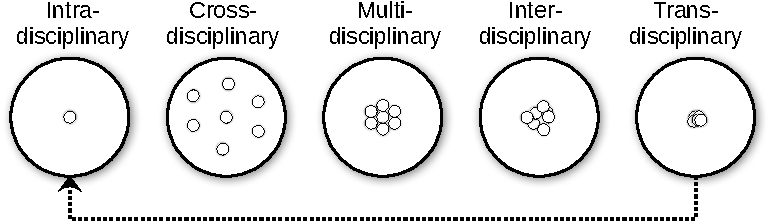
\includegraphics[width=\columnwidth]{figures/01-disciplinarities-crop.pdf}
\caption{A sketch of different levels of disciplinarity, combining the taxonomy of \citet{stember_advancing_1991} with the drawing by \citet{zeigler_dont_1990}. While drawn as separate categories, the different levels should be seen as following each other on a continuum.}
\label{fig:interdisciplinary}
\end{figure}

Identifying the target group is challenging when working interdisciplinary. When writing within a discipline, one may assume familiarity with core concepts and ideas. Throughout the years, I have presented theories from this book to many different audiences. It is remarkable how different responses I get when talking in front of groups of, say, musicologists, psychologists, or computer scientists. It is equally challenging to target groups of composers, performers, or designers. I have seen the need to `translate' terms and explain concepts to fit the various audiences. I try to do the same in this book.


\section{Artistic vs scientific research}

In addition to working between different scientific disciplines, my work is also situated in the arts. I like to think of this as a continuum, as sketched in Figure~\ref{fig:nature-culture}. Unfortunately, art and science are often institutionally separated, although there are some examples of how art and science are connected and even integrated \citep{borgdorrf_conflict_2012}. No doubt, there are different theories, methods, praxes, and outcomes between art and science. However, in my experience, artistic methods can be used to develop new knowledge, and scientific methods can lead to new artworks. Some examples of such intertwined knowledge and art production will be presented in Chapters~\ref{chap:unconventional} and \ref{chap:touchless}.

\begin{figure}[tp]
  \centerline{
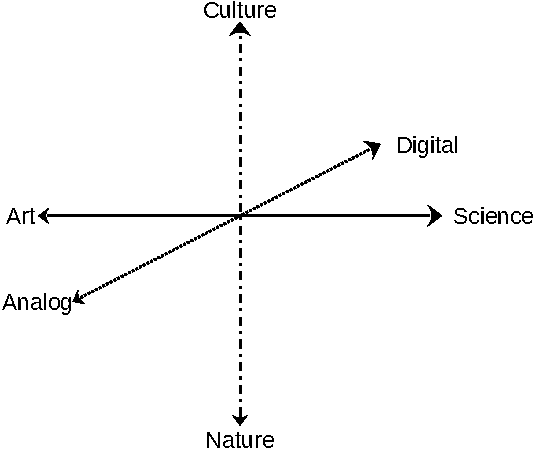
\includegraphics[width=.7\columnwidth]{figures/02-3-axes-crop.pdf}
\caption{This interdisciplinary book project is placed between three (independent) axes: the study of objects along a nature--culture axis, outputs along an art--science axis, and technologies along an analog--digital axis.}
\label{fig:nature-culture}
}
\end{figure}

The second axis in Figure~\ref{fig:nature-culture} is between the humanities (culture) and the natural sciences (nature). Within universities, these traditions are often split into separate faculties. The natural sciences are usually hypothesis-driven, while the humanities are based on hermeneutic interpretation and reasoning. However, there are numerous examples of how humanities scholars use empirical and experimental methods while natural scientists reason and infer. There is also an increased understanding of the need to work in cross-faculty teams to solve the big societal challenges. However, in my experience, that is often easier said than done. Working across faculty borders is challenging at best and impossible at worst. That is probably why most `interdisciplinary' projects end up being cross- or multidisciplinary.

In the third axis in Figure~\ref{fig:nature-culture}, I draw up a separation between analog and digital technologies. There is a tremendous focus on digital technologies these days. Nevertheless, we should not forget all the analog technologies surrounding us, such as door handles, knives, swimming suits, and guitars, to name a few. We should also remember that digital devices have analog components to interface with the analog world. For example, a mobile phone captures and produces sound, light, and vibration. That is why I find it fascinating to investigate the similarities and differences between analog and digital technologies.


\section{Outline of book}

The book is organized into four parts, which each presents one of the project's four main topics:

\begin{description}
  \item[Musicking:] Thinking of music as an active process (`to music'), and how this changes our ideas of instrument making, composition, performance, perception, and analysis. This is also closely connected to questions about musical embodiment and the role of instruments in musical experiences.

  \item[Embodiment:] Defining core terminology from (bio)mechanics and understanding different functions of music-related body motion: from the sound-producing actions to communicative gestures of performers to various types of entrainment and sound-accompanying motion of perceivers.

  \item[Interaction:] Investigating the design and construction of both acoustic and electro-acoustic instruments, and the techno-cognitive differences between action--sound couplings and mappings, their action--sound separation, and the importance of spatiotemporal resolution.

  \item[Affection:] Reflecting on the aesthetic, embodied, and emotional experiences of playing various instruments. Here I will present some of my own prototype instruments and reflect on their design, construction, and performance.
\end{description}

It should be possible to read the individual parts of the book independently, as they each introduce a complete set of conceptual building blocks. To understand their connections, however, it will be necessary to read the book linearly. I also recommend trying out various instruments while reflecting on the presented concepts. After all, musicking is an active and embodied process.
